\section{Problem 2}
\subsection{Implementing KNN}

This is my implementation of KNN
\begin{minted}[linenos, bgcolor = bg, breaklines]{python}
# Calculates the euclidean distance between two points.
def euclidean_distance(x1, x2):
    return np.sqrt(np.sum((x1 - x2)**2))

def __kNNTest(trainingFeatures2D, trainingLabels, n_neighbors, validationFeatures2D, validationLabels):
    # make a counter to count how many times we find the correct label
    count = 0

    # Iterates the length of validationFeatures2D array
    for i in range(np.size(validationFeatures2D,0)):
        # Creates an empty distance array for each new iteration in the validationFeatures2D array
        dist_arr = np.empty(np.size(trainingFeatures2D,0))

        # Iterates the length of trainingFeatures2D array
        for j in range(np.size(trainingFeatures2D,0)):
            # Calculates the distance using the np.linalg.norm
            dist = np.linalg.norm(validationFeatures2D[i] - trainingFeatures2D[j])
            # inserts the calculated distances into the dist_arr
            dist_arr[j] = dist
        # Creates label array, that is sorted using argsort which sort an
        # array returning the indices that holds the lowest value (distance in this case)
        label_arr = dist_arr.argsort()

        # Create new variables to calulate the number of occurences of a specific label
        zero = 0
        one = 0
        two = 0
        pred_label = trainingLabels[label_arr[0]]

        # Check what labels we find in the label array
        for x in range (n_neighbors):
            if trainingLabels[label_arr[x]] == 0:
                zero = zero + 1
            elif trainingLabels[label_arr[x]] == 1:
                one = one + 1
            elif trainingLabels[label_arr[x]] == 2:
                two = two + 1
        # Insert the value into the predicted label array
        if zero > one and zero > two:
             pred_label = 0
        elif one > zero and one > two:
            pred_label = 1
        elif two > zero and two > one:
            pred_label = 2

        # Check if the prediction we made is corrosponding to the one in the validation array
        # if correct, increase the counter by one
        if pred_label == validationLabels[i]:
            count = count + 1

    # calucate the final count of corret labels in order to return it as a float (reprecenting accuracy in %)
    accuracy = count / len(validationFeatures2D)
    return accuracy

for n in range(1, 6):
    print('accuracy = ', __kNNTest(trainingFeatures2D, trainingLabels, n, validationFeatures2D, validationLabels))

\end{minted}

\begin{figure}[H]
    \centering
    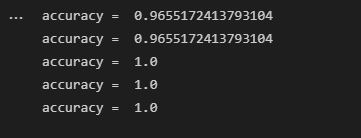
\includegraphics[width=0.75\textwidth]{Figures/KNN_result.JPG}
    \caption{result of the KNN algorithm}
\end{figure}

In the picture, we can see the accuracy of the KNN algorithm, when looking at the
n'th nearest neighbors. The first value is when looking at 1 neighbor, and the last one
is when looking at the 5 nearest neighbors.
This means, that the more neighbors the algorithm takes into consideration, the more accurate it
can predict which classification the given point should have.
